\documentclass{article}

%%%%
% PLOTS mapas
% eval=FALSE
% results=HIDE (verbatim default)
%%%%
\usepackage[utf8]{inputenc}
\usepackage{longtable}
\usepackage{authblk}
\usepackage{adjustbox}

%%%%
\usepackage{Sweave}
\begin{document}
\Sconcordance{concordance:basico32departamentos.tex:basico32departamentos.Rnw:%
1 18 1 1 9 2 1 1 31 6 1 1 12 1 4 1 1 1 12 1 5 1 1 1 27 4 1 1 27 1 2 16 %
1}



%Partes extras para las nuevas columnas
% Exploracion Univariada --------------------------------------------------

\section{Exploración Espacial}

Estos son los lugares donde tenemos información:



%con esto hagamos el merge:



 
 
\begin{figure}[h]
\centering
\begin{adjustbox}{width=18cm,height=13cm,clip,trim=1.5cm 2cm 0cm 2.5cm}
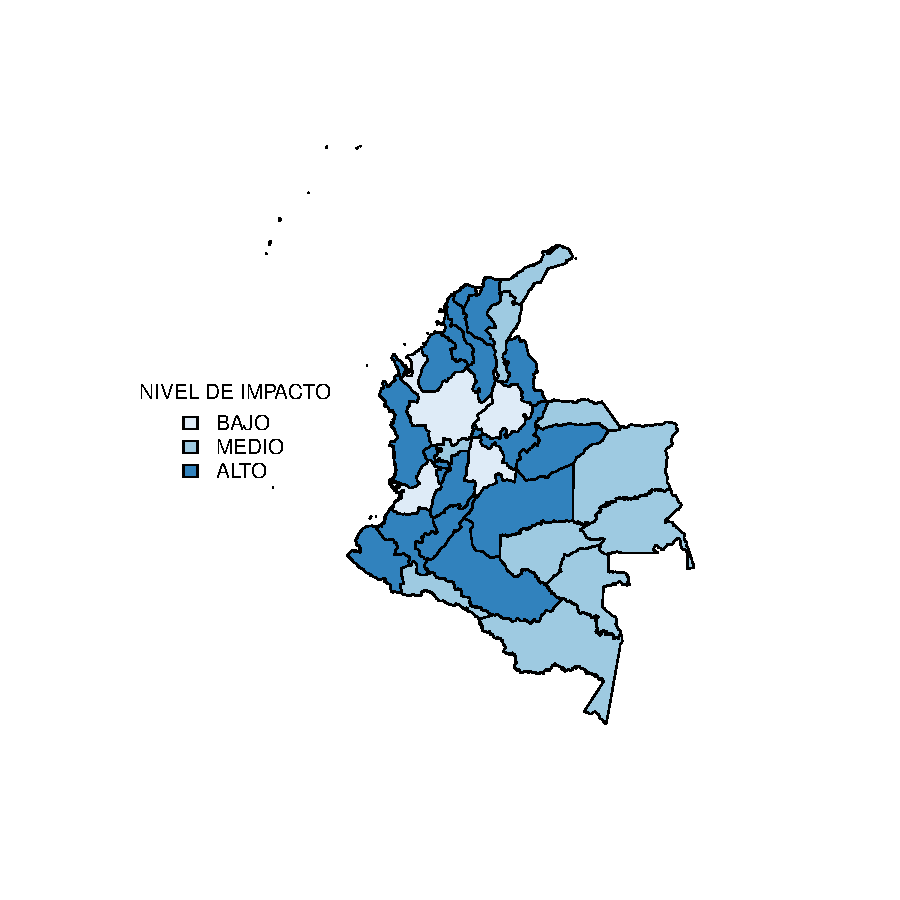
\includegraphics{basico32departamentos-plotMap0}
\end{adjustbox}
\caption{Departamentos con información diponible}\label{rawmap}
\end{figure}

\end{document}
